\chapter{Вывод формулы максимального размера стека окон в Алгоритме Варнока}
\label{cha:appendix2}

Пусть выполняется рекурсивное разбиение окна на четыре равные части, причём сначала оно разбивается по стороне с максимальной длиной, а затем по стороне с минимальной длиной. Разбиение производится, если длина соответствующей стороны окна больше 1. На рисунке \ref{fig:subdivide_2} показаны примеры таких разбиений.

\begin{figure}[h]
	\centering
	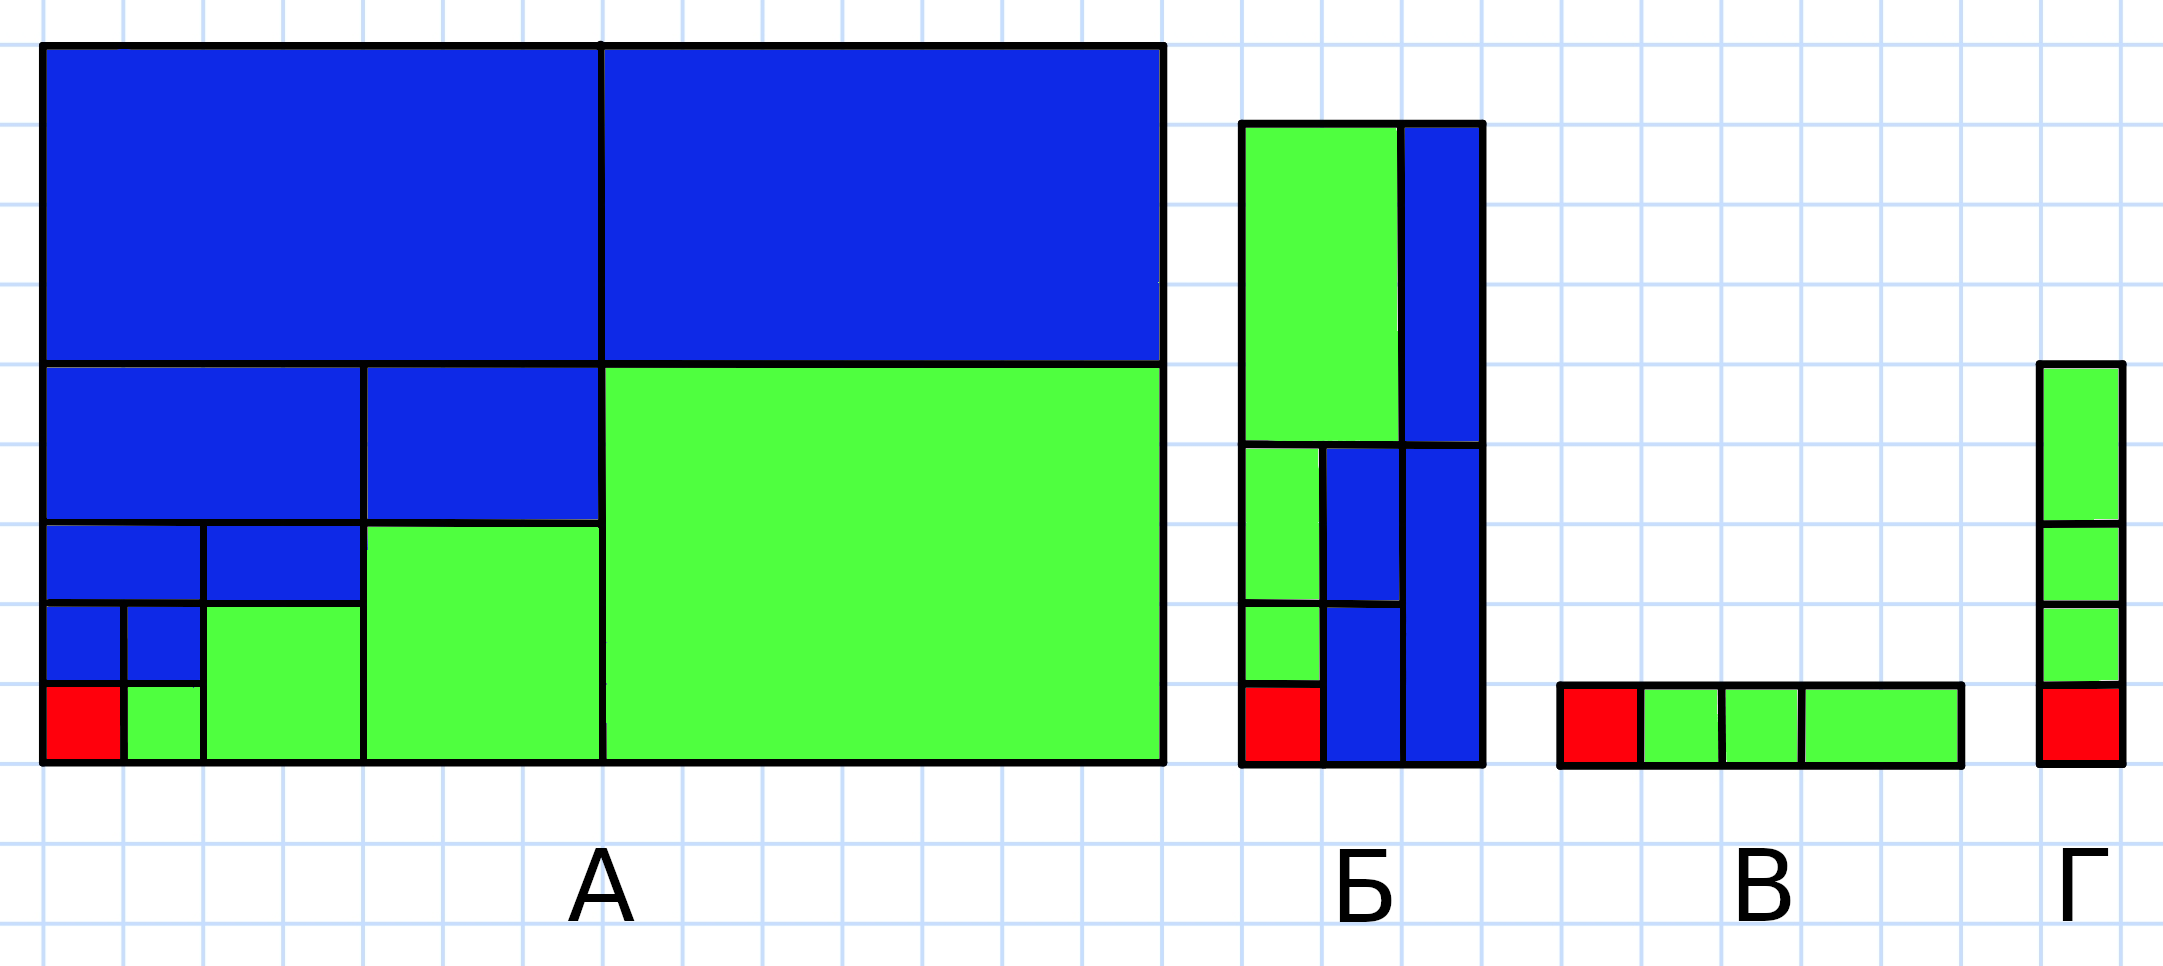
\includegraphics[width=\textwidth ]{img/subdivide_2.png}
	\caption{Примеры разбиения окон в алгоритме Варнока}
	\label{fig:subdivide_2}
\end{figure} 

Подокна, получившиеся в результате разбиения, можно разделить на 3 типа: 

\begin{itemize}
	\item подокна, получившиеся при разбиении окна по стороне с максимальной длиной (в примере отмечены зелёным цветом);
	\item подокна, получившиеся при разбиении окна по стороне с максимальной длиной (в примере отмечены синим цветом);
	\item подокно, имеющее размеры $1\cdot1$ пиксель и являющееся терминатором рекурсии (в примере отмечен красным цветом).
\end{itemize}

Обозначим ширину и высоту исходного окна за $w$ и $h$ соответственно. Тогда максимальное количество разбиений окна по стороне с максимальной длиной будет равно

\begin{equation}
	\label{eq:n_max}
	n_{max} = \lceil\log_{2} (max(w; h))\rceil.
\end{equation}

Количество таких окон будет равно $n_{max}$. Максимальное количество разбиений окна по стороне с минимальной длиной будет равно

\begin{equation}
	\label{eq:n_min}
	n_{min} = \lceil\log_{2} (min(w; h))\rceil.
\end{equation}

Количество таких окон будет равно $2 \cdot n_{max}$. Учитывая единственное подокно, являющееся терминатором рекурсии, максимальный размер стека окон будет равен

\begin{equation}
	\label{eq:res}
	Size = \lceil\log_{2} (max(w; h))\rceil + 2 \cdot \lceil\log_{2} (min(w; h))\rceil + 1.
\end{equation}

%%% Local Variables: 
%%% mode: latex
%%% TeX-master: "rpz"
%%% End: 
